% Beamer Presentation
% Nicholas R. Jenkins (nicholas.jenkins@email.ucr.edu)
% Department of Political Science
% University of California, Riverside
%
% Presentation for: Article_Title
% ---------------------------------------------------------------------------

% Document and Theme Setup %
\documentclass[12pt, aspectratio=169]{beamer}
\usetheme{default}
\usecolortheme{crane}
\useoutertheme[subsection=false, footline=authortitle]{miniframes} 
\usefonttheme{default}  	% default, professionalfonts, serif, structurebold, structureitalicserif, structuresmallcapsserif,
\setbeamercovered{transparent} 
\setbeamertemplate{navigation symbols}{}

% Remove Navigation Dots at the top of the slides %
\makeatletter
\def\beamer@writeslidentry{\clearpage\beamer@notesactions}
\makeatother

% Load Packages %
\usepackage[utf8]{inputenc}
\usepackage[english]{babel}
\usepackage{csquotes}
\usepackage{amsmath}
\usepackage{amsfonts}
\usepackage{amssymb}
\usepackage{graphicx}
\usepackage{bookmark}
\usepackage{appendixnumberbeamer}
\usepackage{tikz}
\usetikzlibrary{positioning}
\usepackage{tabu}
\usepackage{graphicx}
\usepackage{longtable}
\usepackage{booktabs}
\usepackage{amsfonts}
\usepackage{pdflscape}
\usepackage{footmisc}
\usepackage{subfig}
\usepackage{bm}
\usepackage{longtable}
\usetikzlibrary{shapes, shadows, arrows}
\usepackage{rotating}
\usepackage{multirow}
\usepackage[section]{placeins}
\usepackage{pgfplots}


% Define Colors %
% These are the UC Riverside colors found here: http://creativedesign.ucr.edu/ism/colors.html
\definecolor{UCRGray}{RGB}{122, 110, 103}
%\definecolor{UCGold}{RGB}{255, 181, 17} % UC System Color
%\definecolor{UCBlue}{RGB}{18, 149, 216} % UC System Color
\definecolor{UCGold}{RGB}{241, 171, 0} % UC Riverside Official Color
\definecolor{UCBlue}{RGB}{45, 108, 192} % UC Riverside Official Color
\definecolor{UCBlack}{RGB}{0, 0, 0} 
\definecolor{lightgray}{RGB}{215, 215, 215}


% Set Colors %
\setbeamercolor*{palette tertiary}{fg=black, bg=UCGold} % Section color (color of navigation header and dots)
\setbeamercolor{frametitle}{fg=UCBlue, bg=white} % Color of the title bar on each frame
\setbeamercolor{title}{fg=UCBlue, bg=lightgray} 
\setbeamercolor{alerted text}{fg=UCGold} % Color of alert text and block
\setbeamercolor{example text}{fg=UCBlue} % Color of example text
\setbeamercolor{enumerate item}{fg=UCBlue} % Number color
\setbeamercolor{itemize item}{fg=UCBlue} % Bullet point color
\setbeamertemplate{itemize items}[square] % Bullet point style 
\setbeamercolor{button}{bg=lightgray,fg=UCBlue} % Button Color



% University Macros %
\newcommand{\ucr}{Department of Political Science \\ 
University of California, Riverside \\
\textit{nicholas.jenkins@email.ucr.edu}}


% Bibliography Setup %
\usepackage[authordate, natbib, isbn=false, url=false, doi=false, backend=biber]{biblatex-chicago} 
\bibliography{/Users/nickjenkins/Documents/Research/References/BibTeX/biblatex.bib}


% Title Page Information %
\title[Rejecting PACs and Contribution Patterns]{Transparency or Deception? How Rejecting PAC Contributions Affects Contribution Patterns}
%\subtitle{Subtitle}

% Single Author
\author{Nicholas R. Jenkins}
\institute{\ucr}

% Multiple Authors
%\author[Nick]{Nicholas R. Jenkins \inst{1} \and author2 \inst{2}} 
%\institute[shortinst]{\inst{1} \ucr \and \inst{2} affiliation for author2}

\date{\today}


%\subject{} 

% Title Page and Graphics %
\pgfdeclareimage[height=2cm]{university-logo}{UCR-3.png} % Choose UCR-1, UCR-2, UCR-3, or UCR-4 for a logo on each slide
\titlegraphic{\hfill
\includegraphics[height=2cm]{UCR-3}} % Title Page Logo
%\logo{\pgfuseimage{university-logo}} % Logo on Each Slide


% Begin Presentation %
\begin{document}


% Title Page
\begin{frame}
\titlepage
\end{frame}


\section{Motivation} \label{sec: motivation}

\begin{frame}{Motivation}
		\begin{tikzpicture}
		\node (1) at (4,12) {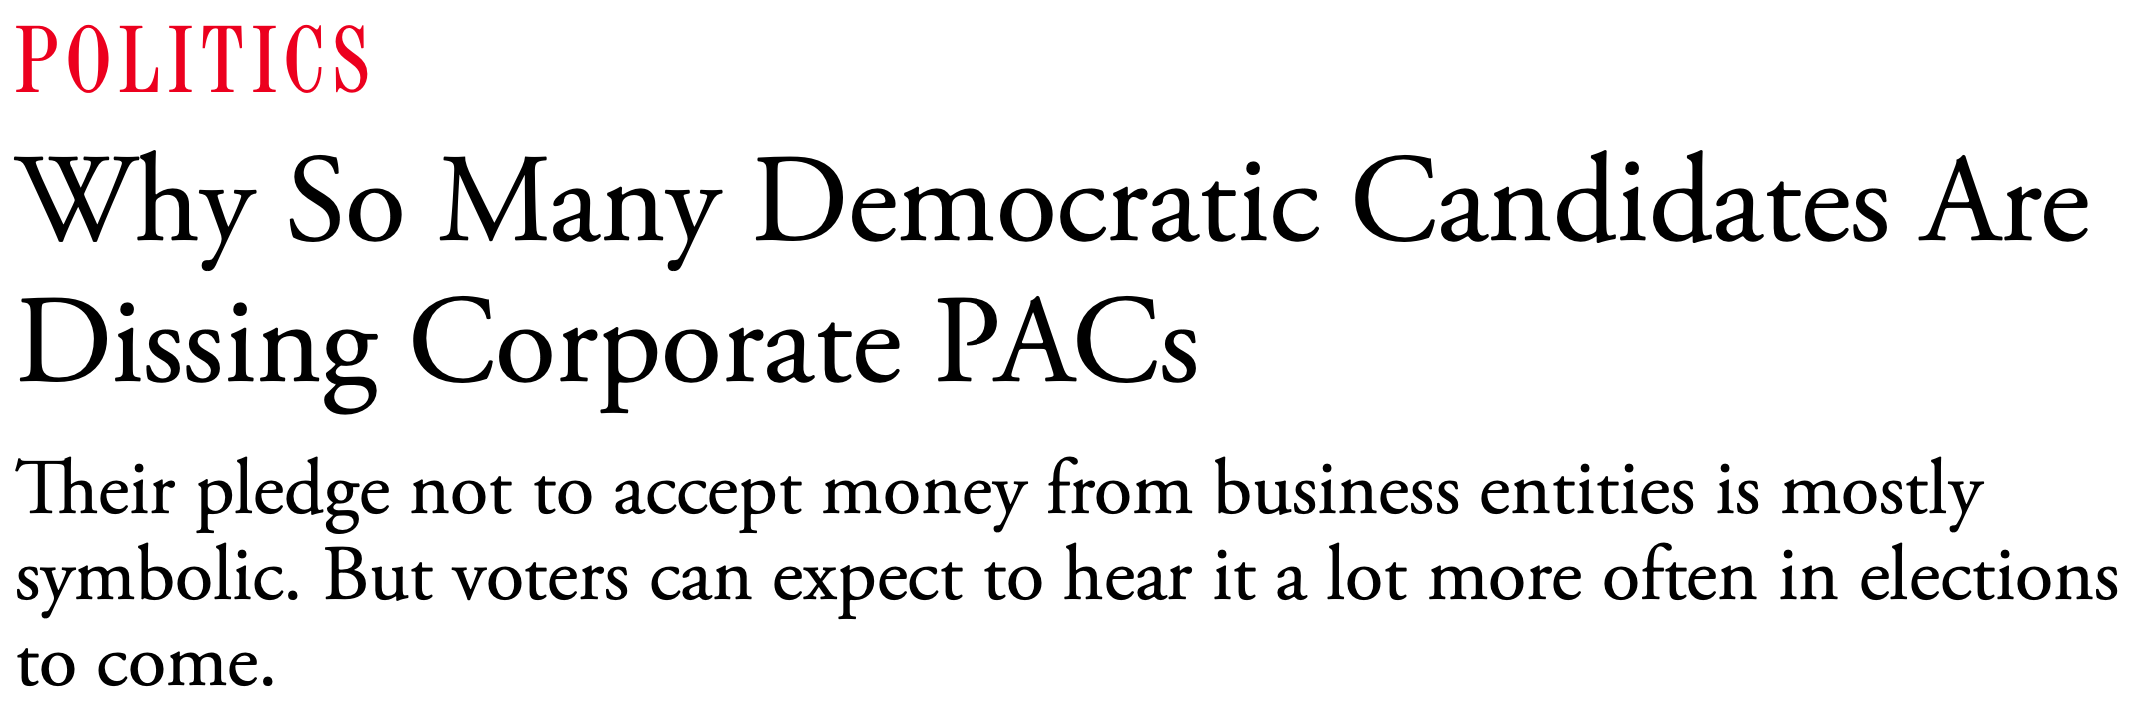
\includegraphics[width=0.7\linewidth]{5}}; 
		\node (3) at (2,6) [yshift=2cm] {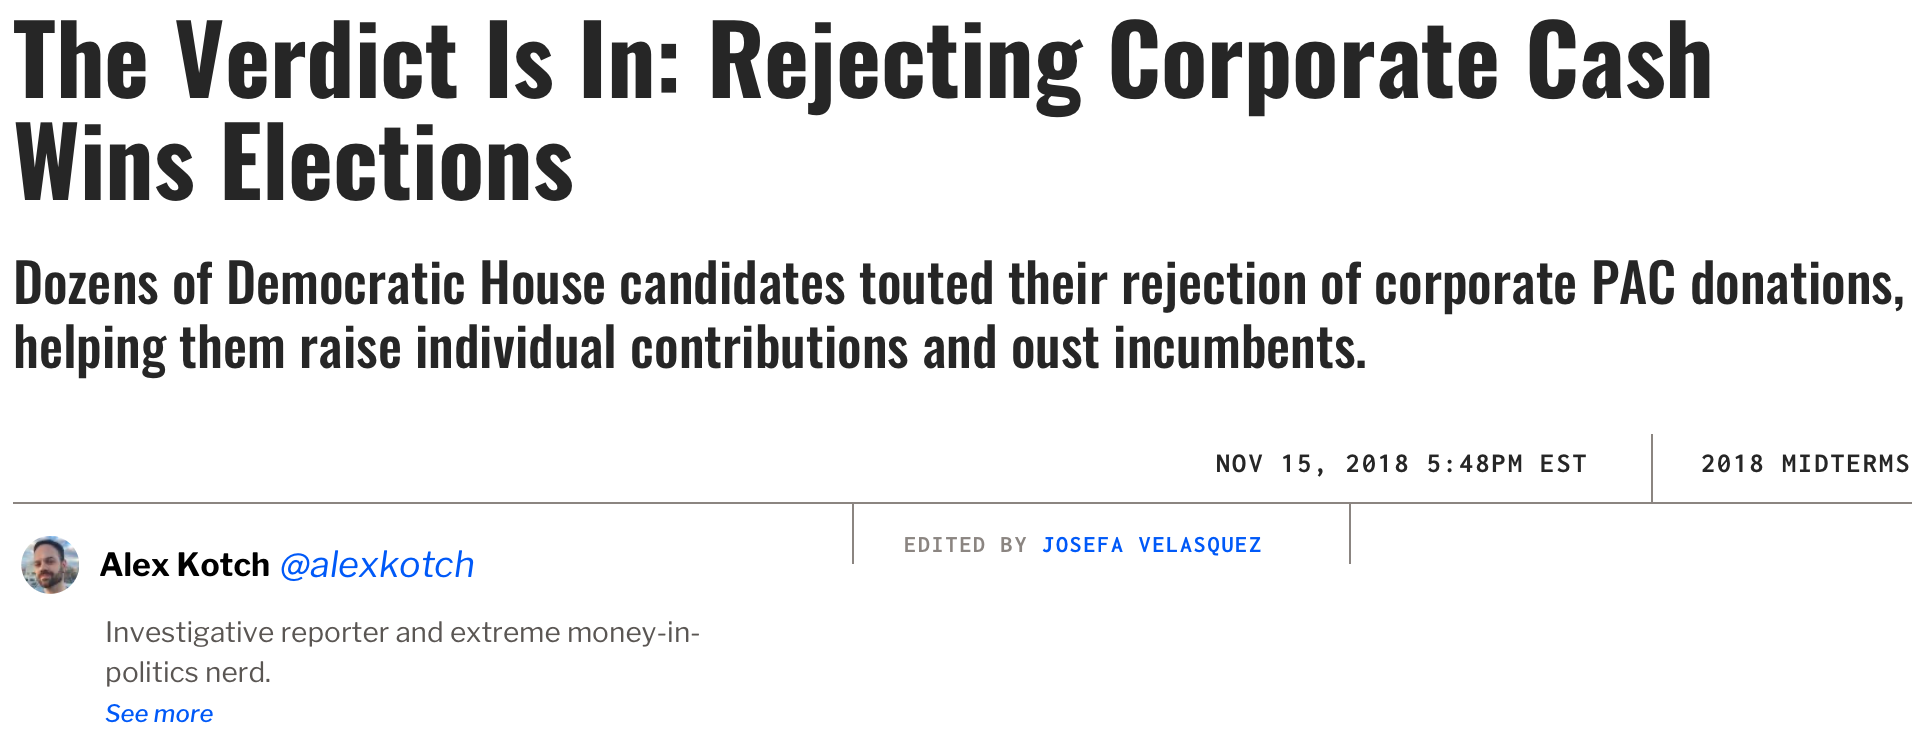
\includegraphics[width=0.6\linewidth]{3}}; 
	\end{tikzpicture}
\end{frame}


\section{Motivation} \label{sec: motivation}

\begin{frame}{Motivation}
		\begin{tikzpicture}
		\node (2) at (-1,8.3) [yshift=2cm] {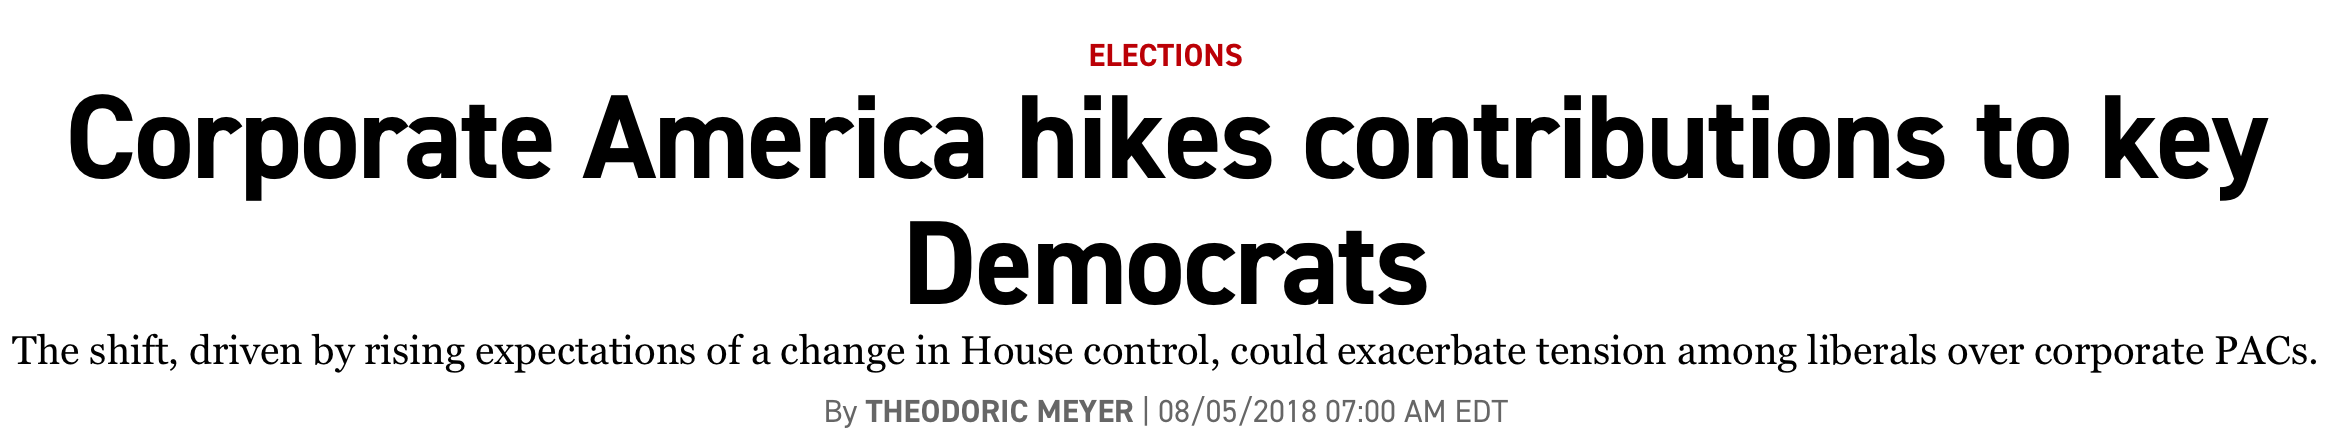
\includegraphics[width=0.6\linewidth]{2}};
		\node (2) at (0,4) [yshift=2cm] {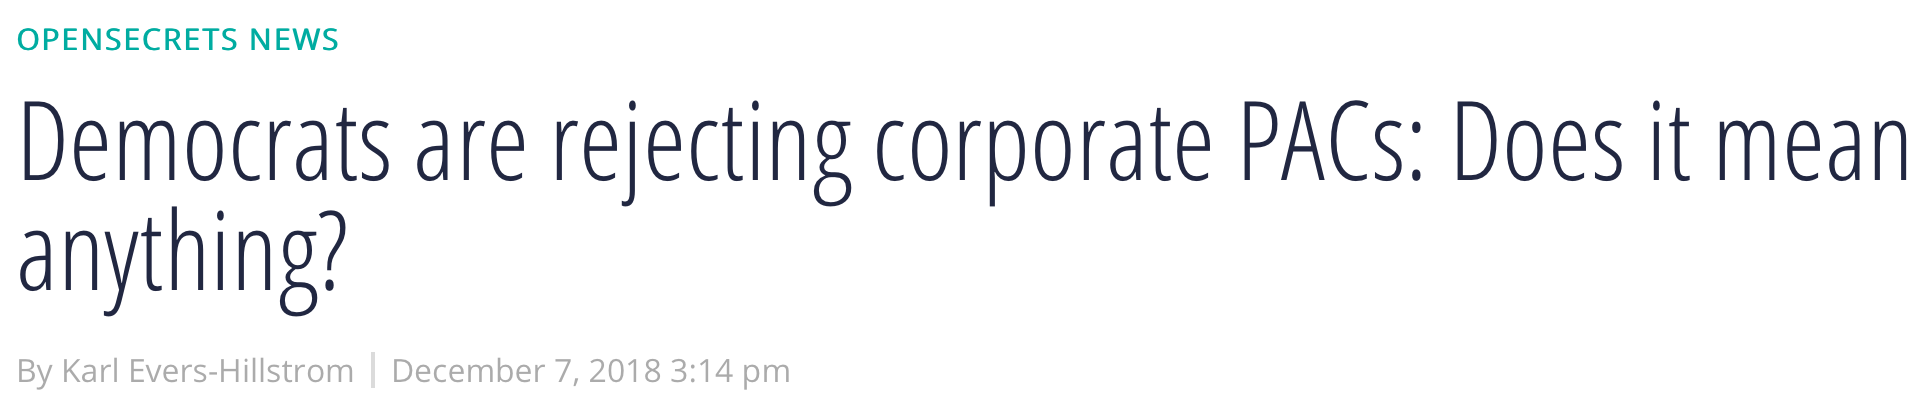
\includegraphics[width=0.6\linewidth]{1}};
		\node (2) at (4,6) [yshift=2cm] {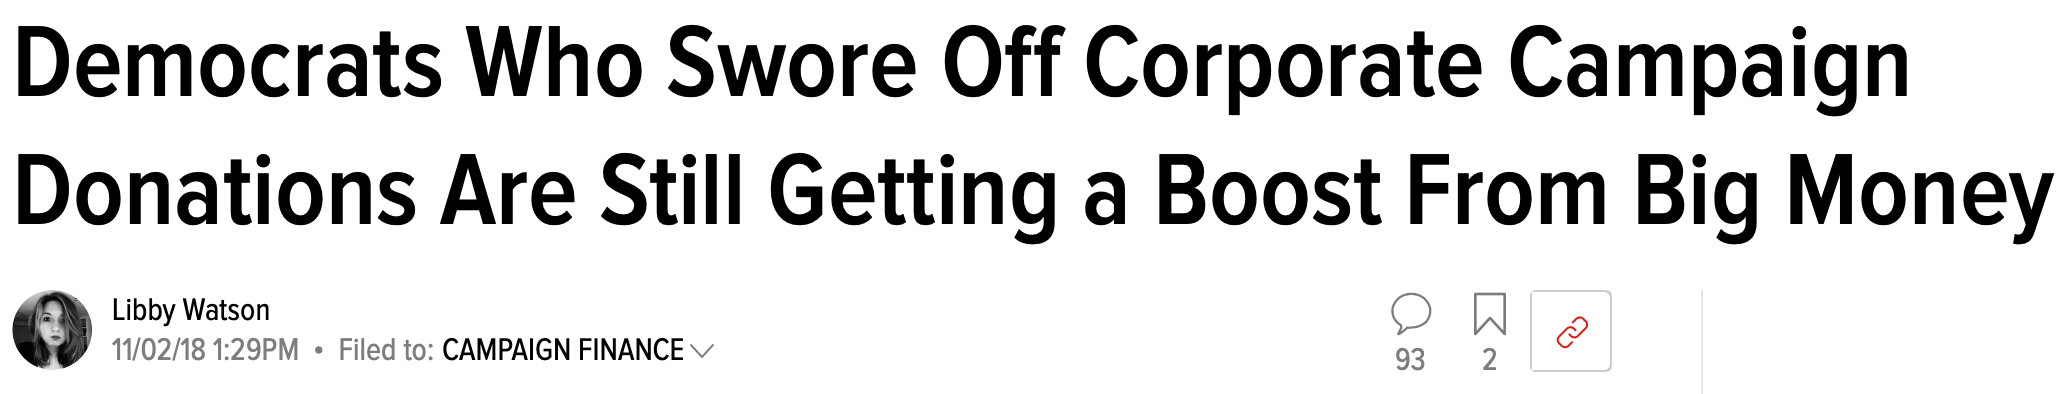
\includegraphics[width=0.6\linewidth]{4}};
	\end{tikzpicture}
\end{frame}

% Table of Contents Slide
%\begin{frame}
%\tableofcontents
%\end{frame}

\begin{frame}{Motivation}
	\begin{alertblock}{Research Question}
		Do pledges to reject corporate PAC contributions minimize corporate influence in elections?
	\end{alertblock}
\end{frame}


\section{Voter Perceptions of Corporate Influence} \label{sec: framework}

\begin{frame}{Why do candidates refuse corporate PAC money?}
	\begin{itemize}
		\item Americans are very skeptical about money in politics {\tiny \citep{lubenow2001}} \pause
		\item Voter believe contributions from corporations are more corrupt than those from other sources {\tiny {\citep{bowler2016}}} \pause
		\item Voters also think that small-dollar contributions are the most trustworthy
	\end{itemize}
\end{frame}

\begin{frame}{Why do candidates refuse corporate PAC money?}
	\begin{itemize}
		\item It's probably strategic! \pause
		\item Elizabeth Warren ``swore off PAC money to make a statement” {\tiny {\citep{nilsen2019}}} \pause
		\item The Democrats in the 2020 presidential race were almost in a competition to distance themselves from corporations 
	\end{itemize}
\end{frame}
% “For every time you see a presidential candidate talking with voters at a town hall, rally, or local diner, those same candidates are spending three or four or five times as long with wealthy donors — on the phone, or in conference rooms at hedge fund offices, or at fancy receptions and intimate dinners — all behind closed doors”

\begin{frame}{Do corporations just give up?}
	\begin{itemize}
		\item Campaigns are extremely expensive! \pause
		\item A lot of opportunity cost to not get involved {\tiny \citep{denzau1986, kroszner1998}} \pause
		\item Corporations bundle individual contributions \pause
		\item ``In some cases, a cluster of contributions from the same organization may indicate a concerted effort by that organization to ‘bundle’ contributions to the candidate” {\tiny \citep{opensecrets.org}}
	\end{itemize}
\end{frame}
% To put this into context, contributions to all candidates from business PACs totaled $394 million in the 2018 election cycle compared to over $1.6 billion from individuals affiliated with business interests (Opensecrets.org 2021). This type of giving strategy would allow recipients to claim that they do not accept corporate PAC money while still receiving corporate support.
% Candidates who adopt this strategy likely do so either because they feel confident that they can win without corporate PAC support or adequately compensate for the loss of funds with those from other sources. “Other sources” could be small-dollar donations, party organizations, or super PACs. Small-dollar donations, however, are unlikely to be substantial enough for most candidates to win or even give them an assurance of a winning strategy. Moreover, given the incentives for corporations to participate in politics, they will likely find alternative means to finance their preferred candidates.

\section{Data}

\begin{frame}{Estimation Sample}
	\begin{itemize}
		\item Campaign finance data on the 2018 midterm election from OpenSecrets.org \pause
		\item 259 Members, 24\% freshman 19\% refuse corporate PAC contributions \pause
		\item Among those who reject corporate PAC contributions: 35 are freshman and 29 are returning members
	\end{itemize}
\end{frame}

\begin{frame}{DW-NOMINATE Scores}
	\begin{figure}
		\centering
		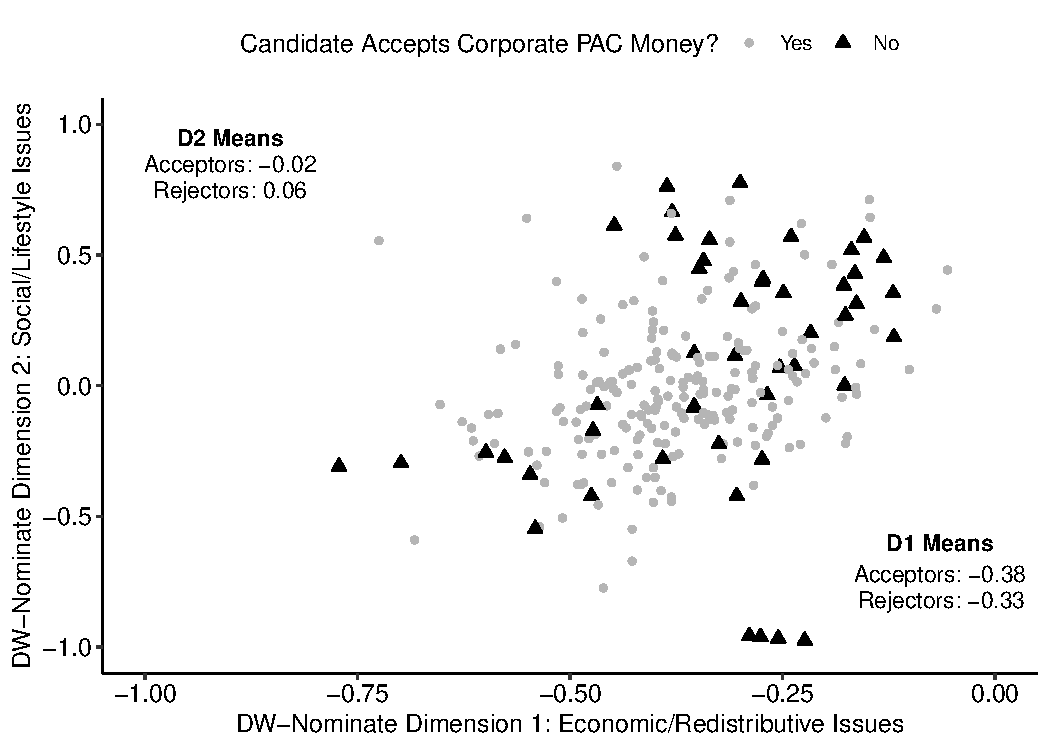
\includegraphics[width=0.65\linewidth]{../Figures/nominate_plot.pdf}
	\end{figure}
\end{frame}

\begin{frame}{Estimation Sample}
	\begin{itemize}
		\item My focus is on contributions from: \pause
		\begin{itemize}
			\item Business PACs \pause
			\item Small-dollar individual contributions \pause
			\item Contributions of \$1,000 or more from individuals who work in business industries \pause
			\item Contributions of \$1,000 or more from individuals who work in business industries and live outside of the member's district \pause
		\end{itemize}
	\end{itemize}
\end{frame}

\begin{frame}{Estimation Sample}
	\begin{figure}
		\centering
		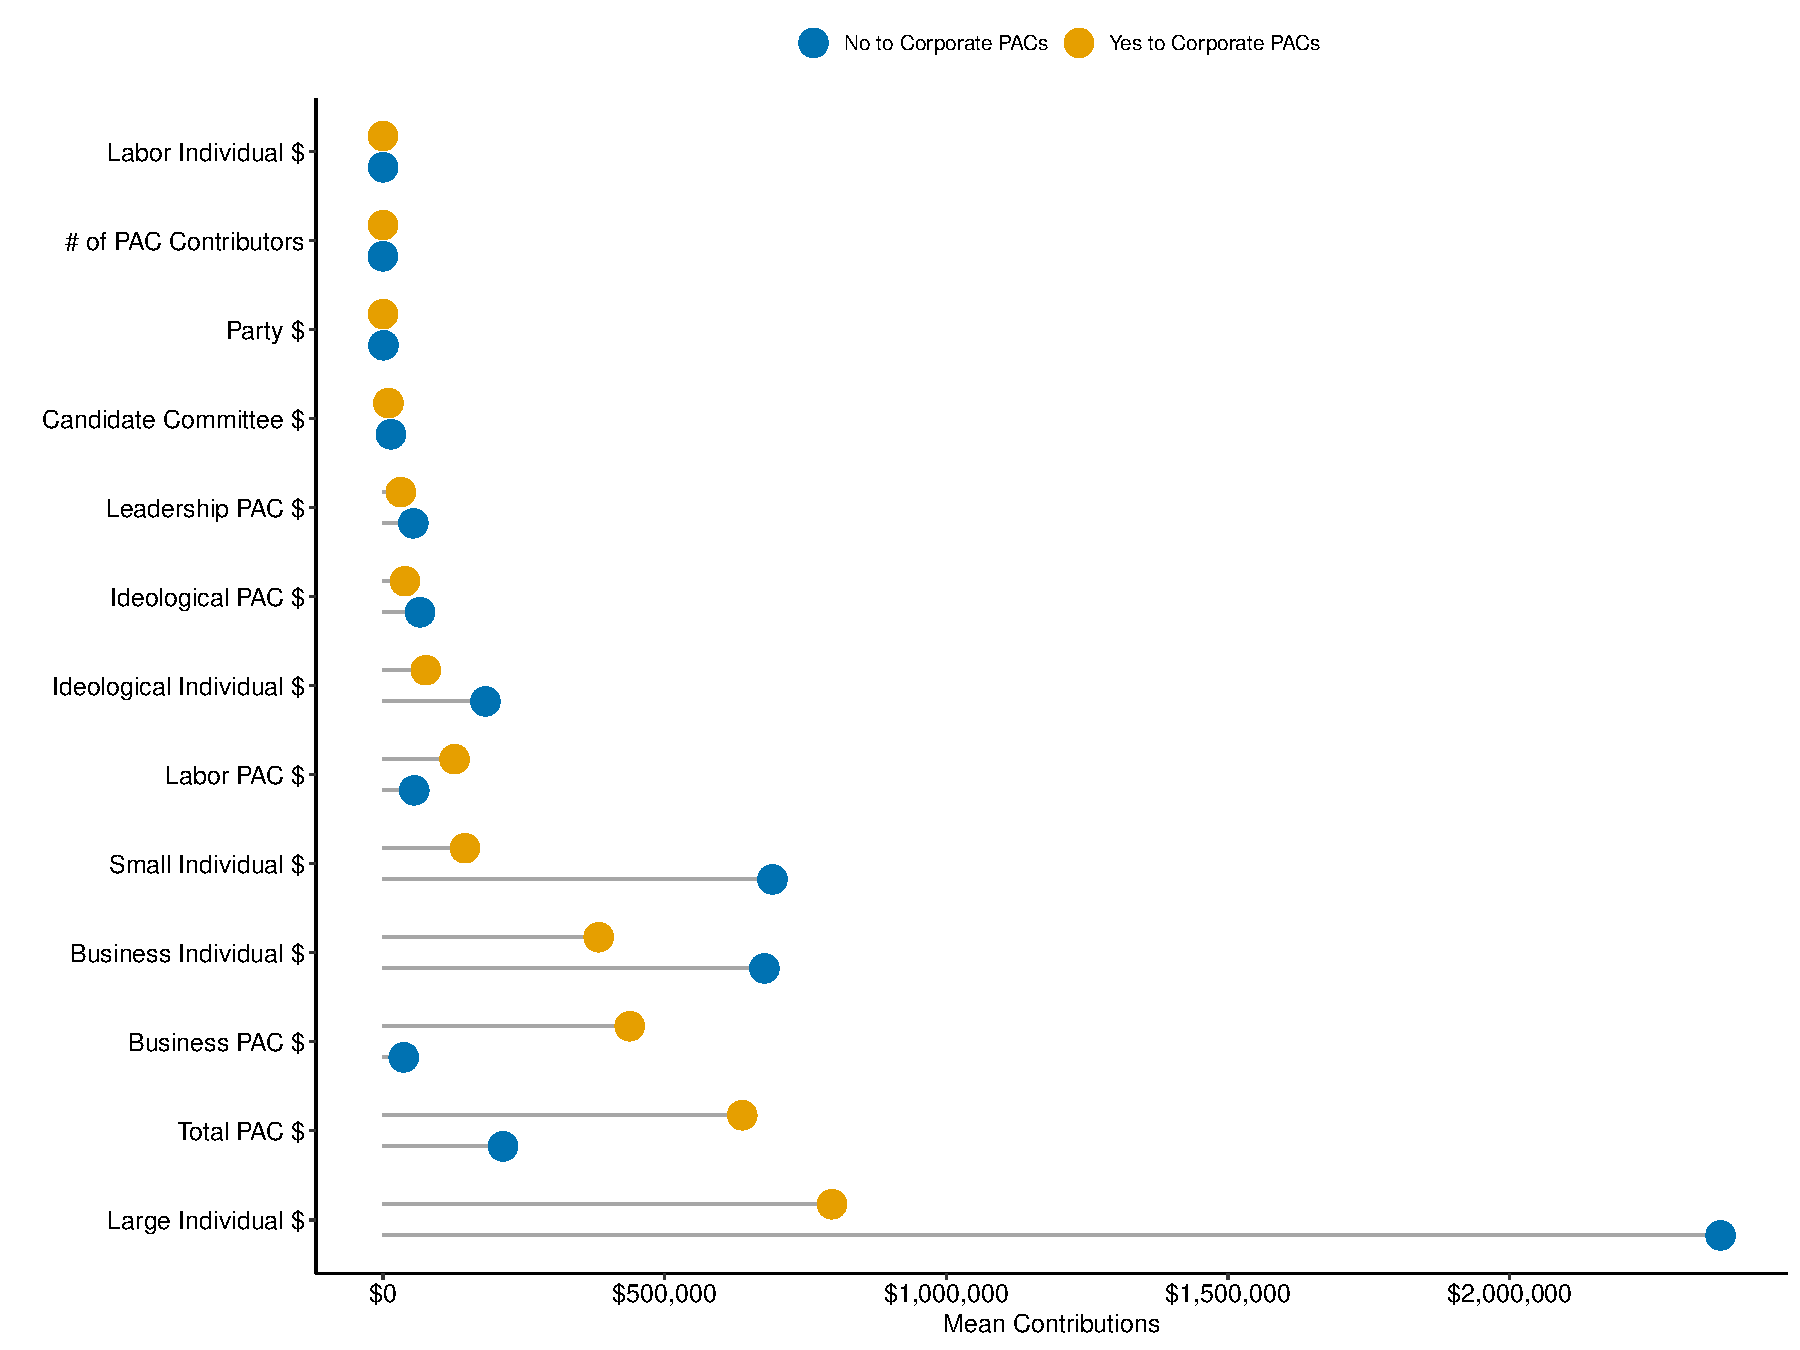
\includegraphics[width=\linewidth]{../Figures/all_candy.pdf}
	\end{figure}
\end{frame}


\section{Methods}

\begin{frame}{How the composition of a member's campaign contribution courses change in response to making an anti-corporate PAC pledge?}
	\begin{itemize}
		\item Outcome Variable: the proportion of contributions received by a candidate from business PACs, business individual, small-dollar, and out-of-district business donations \pause
		\item Predictor of interest: Whether the candidate refuses corporate PAC contributions \pause
		\item Dirichlet likelihood \pause
		\item Controls: New member, district demographics, Democratic vote share, and median household income
	\end{itemize}
\end{frame}


\section{Results}

\begin{frame}
	\begin{figure}
		\centering
		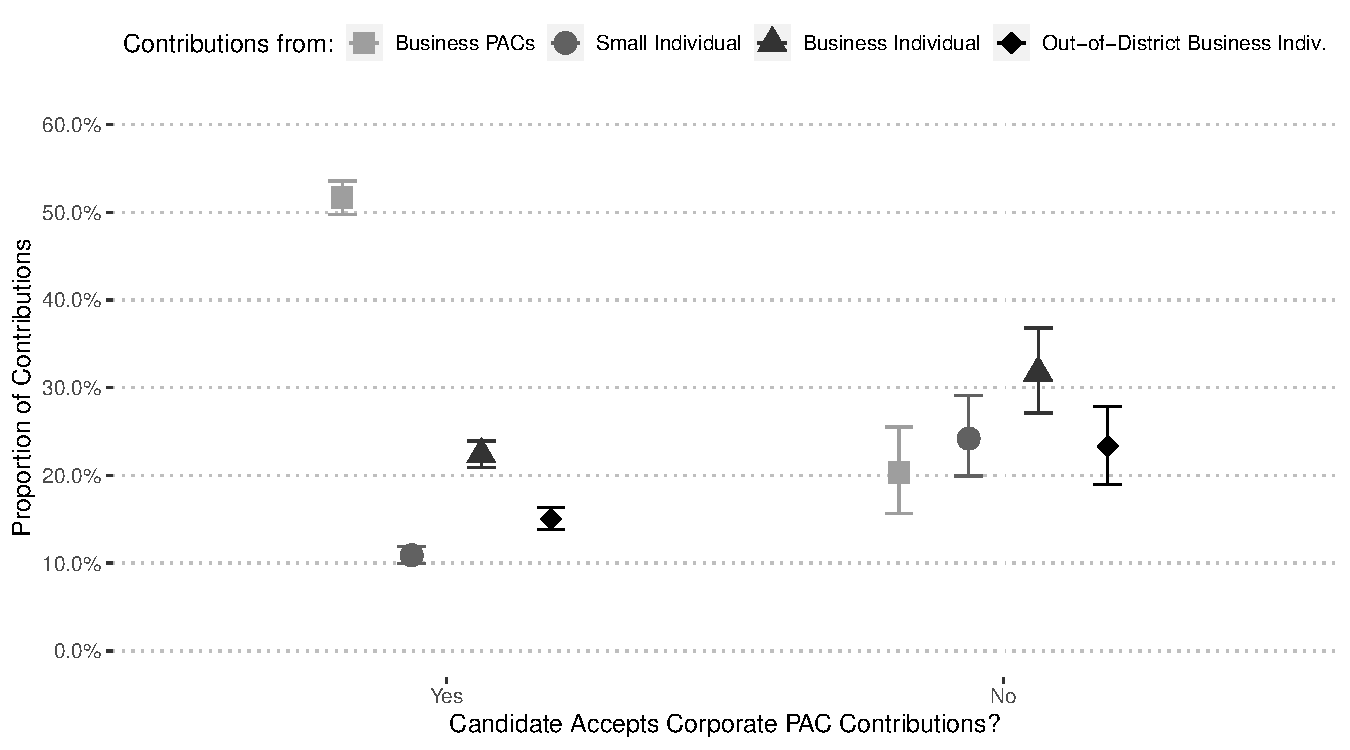
\includegraphics[width=0.95\linewidth]{../Figures/dir_model_results.pdf}
	\end{figure}
\end{frame}
% Candidates who accept corporate PAC contributions are estimated to receive over 50 percent of contributions from business PACs compared to around 20 percent for candidates who refuse them
% In addition to this expected decrease in business PAC contributions, candidates who pledge to reject corporate PAC contributions receive a higher proportion of contributions from small-dollar, business, and out-of-district business individual contributions
% The largest proportional shift is for contributions from small-dollar individuals. Candidates who accept corporate PAC contributions are predicted to receive just over 10 percent of their contributions from small-dollar donors compared to around 25 percent for candidates who refuse corporate PAC money. Similarly, candidates who refuse corporate PAC contributions are predicted to receive around 30 and 25 percent of their contributions from business (contributions from individuals that work in a business industry of $1,000 or more) and out-of-district business individual contributions.


\section{Summary}

\begin{frame}{Summary}

Findings
	\begin{itemize}
		\item Candidates who refuse corporate PAC contributions receive:
		\begin{itemize}
			\item more contributions from small-dollar donors \pause
			\item more contributions from business individuals \pause
			\item more contributions from out-of-district business individuals \pause
		\end{itemize}
	\end{itemize}
	
Implications \pause
	\begin{itemize}
		\item May create a less transparent campaign finance system \pause
		% If public opinion on PAC contributions sours, the organizations these PACs represent may resort to less transparent strategies like the use of super PACs, 527 committees, and “dark money;” indeed emerging evidence suggests that this is already happening
		\item Who is represented with money from other districts?
	\end{itemize}
\end{frame}

\end{document}